\documentclass[10pt]{article}
\usepackage[utf8]{inputenc}
\usepackage[T1]{fontenc}
\usepackage{amsmath}
\usepackage{amsfonts}
\usepackage{mathrsfs}
\usepackage{amssymb}
\usepackage[version=4]{mhchem}
\usepackage{stmaryrd}
\usepackage{bbold}
\usepackage{enumitem}
\usepackage{hanging} %reference indent
\usepackage[a4paper,left=25mm,right=25mm,top=40mm,bottom=40mm]{geometry}
\usepackage{sectsty}
\sectionfont{\fontsize{10}{15}\selectfont}
\subsectionfont{\fontsize{10}{15}}
\usepackage[mathlines,switch]{lineno}
\usepackage{amsthm}
\usepackage{kotex}
\usepackage{xcolor}
\usepackage{graphicx} % insert image
\usepackage{multicol} % multi column
\usepackage{algorithm}
\usepackage{algpseudocode}
\usepackage{float}
\usepackage{tabularx}
\usepackage{multirow} % multirow in table
\usepackage{tikz}
\usepackage{subcaption}
\usepackage{hyperref}
\usepackage[inkscapeformat=png]{svg}
\modulolinenumbers[5]
% \linenumbers

\usepackage{titlesec}
\titleformat{\section}
{\normalfont\fontsize{12}{12}\bfseries}{\thesection}{1em}{}
\titleformat{\subsection}
{\normalfont\fontsize{11}{11}\bfseries}{\thesubsection}{1em}{}
\titlespacing{\paragraph}{0pt}{\parskip}{5pt}
\titleformat{\title}
{\normalfont\fontsize{13}{13}\bfseries}{\thetitle}{1em}{}

\usepackage{indentfirst} % first line indent
\setlength{\parindent}{10pt}

\renewcommand{\arraystretch}{1.1}

\title{
\textbf{Learning semi-Markovian DAGs with flow-based VAE}}

\author{\normalsize\bfseries Dangchan Kim, Byungguk Kang, Jaeseok Kim, Minchan Kim}

\begin{document}
\maketitle

\begin{abstract}
    We propose a method to learn the structure of a semi-Markovian directed acyclic graph, which is a mixed graph containing both directed and bidirectional edges, using a flow-based variational autoencoder. The proposed method is based on the assumption that noise variables in the linear structural equation model can be considered as latent variables. To learn the structure of the mixed graph, we employ an inverse autoregressive flow to approximate the dependency structure of the noise variables and its prior distribution. We conducted experiments on simulated data by adjusting the number of nodes and the proportion of bidirectional edges. The code is available at \url{https://github.io/ddangchani/NFG-VAE}.
\end{abstract}

\section{Introduction}

Directed acyclic graphs (DAGs) are commonly used to represent causal relationships between variables \cite{pearl_2009}. However, recovering the causal structure from observational data is an NP-hard problem \cite{ChickeringNPhard}. To overcome this problem, several methods have been proposed. NOTEARS \cite{zheng2018dags} is a method that learns the structure of DAGs by minimizing the continuous approximation of the discrete constraint, enabling the learning of DAGs through continuous optimization.\\

Based on the continuous acyclicity constraint neural network-based approaches known as graph neural networks, have been proposed. \cite{yu2019daggnn,li2020dirichlet,kipf2016variational,zhang2019dvae} The most representative model would be DAG-GNN \cite{yu2019daggnn}, a method that learns the structure of DAGs by using a neural network that takes the adjacency matrix of the graph as an additional input. It utilizes a variational autoencoder (VAE) to learn DAGs by interpreting the noise variable in the linear structural equation model as a latent variable.\\

However, in some cases, the noise variables may not be independent. For example, in a linear structural equation model with correlated hidden variables, the noise variables may exhibit a dependency structure. In such cases, edges with correlation in the noise variable are considered bidirectional edges, and these models are referred to as semi-Markovian \cite{Shipster2006semimarkovian}. Since the prior distribution of the noise variable is assumed to be a standard Gaussian in DAG-GNN or other graph neural networks, it becomes challenging to learn the structure of semi-Markovian DAGs. Therefore, we propose a method to learn the full covariance matrix of the noise variable using a flow-based VAE.

\section{Directed Acyclic Graphs and Mixed Graphs}
\subsection{Directed Acyclic Graphs}

Here is the introduction of DAGs

\subsection{Mixed Graphs}

Here is the introduction of mixed graphs

\subsection{Graph Learning}

Here is the introduction of graph learning

\section{Variational Autoencoders and Normalizing Flows}

\subsection{Variational Autoencoders}

VAE(Variational Auto-Encoder)\cite{kingma2013auto} is a neural network architecture that consists of a generative model and a variational inference. In VAE architecture, it is assumed that the continuous latent variable exists and its posterior probability is intractable. Therefore, variational inference is introduced to approximate the real posterior probability with ELBO(evidence lower bound).\\

Let $x$ be an observed variable and $z$ be a latent variable. $x$ is generated by some random process involving $z$. For parameter $\theta$, random variable $z$ is generated from prior distribution $p_{\theta}(z)$, then $x$ is generated from conditional distribution $p_{\theta}(x|z)$. And $p_{\theta}(x,z)$ becomes their parametric joint distribution. Given a dataset $\mathsf{X} = \{ x^{(1)}, ... , x^{(N)}\}$, maximum marginal likelihood learning is to maximize log likelihoods $\log{p_{\theta}(\mathsf{X})} = \sum_{i=1}^{N}{\log{p_{\theta}(x^{(i)})}}.$ However, marginal likelihood $p_{\theta}(x) = \int{p_{\theta}(z)p_{\theta}(x|z)dz}$ is intractable in general. Instead, we introduce the model parameter $\phi$ and a parametric inference model $q_{\phi}(z|x).$ Then we can reformulate the original log likelihoods with $q_{\phi}(z|x).$ \\
\begin{equation*}
	\begin{aligned}
		\log{p_{\theta}(x)} =  \mathbb{E}_{q_{\phi}(z|x)}\left[ \log{p_{\theta}(x)} \right] &= \mathbb{E}_{q_{\phi}(z|x)}\left[ \log{p_{\theta}(x)} + \log{p_{\theta}(z|x)} - \log{p_{\theta}(z|x)} \right] \\
		&= \mathbb{E}_{q_{\phi}(z|x)}\left[ \log{p_{\theta}(x, z)} - \log{q_{\phi}(z|x)} \right] + \mathbb{E}_{q_{\phi}(z|x)}\left[ \log{q_{\phi}(z|x)} - \log{p_{\theta}(z|x)} \right] \\
	\end{aligned}
\end{equation*}
\\

The second RHS term of the last equation is the KL divergence of the approximate posterior from the true posterior. Since KL divergence is non-negative, the first RHS term of the last equation can be expressed as $\mathcal{L}(\theta, \phi; x)$ and it is called variational lower bound.
\begin{equation*}
	\begin{aligned}
	\mathcal{L}(\theta, \phi; x) &= \mathbb{E}_{q_{\phi}(z|x)}\left[ \log{p_{\theta}(x, z)} - \log{q_{\phi}(z|x)} \right] \\
	\log{p_{\theta}(x)} &= \mathcal{L}(\theta, \phi; x) + D_{KL}( q_{\phi}(z|x) || p_{\theta}(z|x)) \geq \mathcal{L}(\theta, \phi ; x) \\
	\end{aligned}
\end{equation*}
\\
Therefore $\mathcal{L}(\theta, \phi; x)$ is the lower bound of the evidence, marginal likelihood. Under some condition of the distribution family $\{ q_{\phi} \}, $ maximizing $\mathcal{L}(\theta, \phi; x)$ with respect to $\{ \theta, \phi \}$ will simultaneously maximize log-likelihood $\log{p_{\theta}(x)}$ and minimize $ D_{KL}( q_{\phi}(z|x) || p_{\theta}(z|x))$. In VAE architecture, we set $\mathcal{L}(\theta, \phi; x)$ as objective function to be maximized.\\

The ELBO also can be written as 
\begin{equation*}
	\begin{aligned}
		\mathcal{L}(\theta, \phi ; x) &= -\mathbb{E}_{q_{\phi}(z|x)}\left[ \log{q_{\phi}(z|x)} - \log{p_{\theta}(z)} - \log{p_{\theta}(x|z)}  \right] \\
		&= -D_{KL}( q_{\phi}(z|x) || p_{\theta}(z)) + \mathbb{E}_{q_{\phi}(z|x)}\left[ \log{p_{\theta}(x|z)}  \right]. \\
	\end{aligned}
\end{equation*}

To estimate the lower bound, sampling method is used. However, Monte Carlo estimate of the expectation over $q_{\phi}(z|x)$ should be differentiable with respect to $\phi$ in gradient method. Reparametrization trick is introduced to solve this problem. It is often possible to express random variable $z \sim q_{\phi}(z|x) $ as a deterministic variable $z = g_{\phi}(\epsilon, x)$ for auxiliary variable $\epsilon \sim p(\epsilon)$. This reparametrization moves the uncertainty induced by $\phi$ into $\epsilon$ and makes the whole estimation differentiable.

\subsection{Normalizing Flows}

Normalizing flows are a method of transforming a simple distribution into a complex distribution \cite{rezende15normalizingflows}. Let $z$ be a random variable with a simple distribution $p(z)$, and $x$ be a random variable with a complex distribution $p(x)$. We can transform $z_0$ into $z_T$ using a series of invertible transformations $\{f_k\}_{k=1,\ldots,T}$ as follows:
\begin{equation}
    z_T = f_T \circ f_{T-1} \circ \cdots \circ f_1(z_0)
\end{equation}

The probability density function of $x$ can be obtained by the change of variables formula:
\begin{equation}
    p(z_T) = p(z_0) \left| \det \left( \frac{\partial f_T \circ f_{T-1} \circ \cdots \circ f_1(z_0)}{\partial z_0} \right) \right|
\end{equation}

In VAE, the prior distribution of the latent variable $\mathbf{z}$ is typically assumed to be a standard Gaussian distribution or a multivariate Gaussian distribution with a diagonal covariance matrix. \cite{kingma2013auto} However, to employ a more flexible prior distribution, we can utilize normalizing flows to transform the standard Gaussian distribution into a more complex distribution. This allows us to capture richer and more intricate patterns in the latent space, such as correlation between latent variables.\\

There are several types of normalizing flows, such as Householder flow \cite{tomczak2017householder}, planar flow \cite{rezende15normalizingflows}, etc. In this paper, we use the inverse autoregressive flow (IAF) \cite{kingma2016iaf}, especially linear IAF. The linear IAF is defined as follows:

\begin{equation}
    \bf z_t = \bf \mu_t + \bf \sigma_t \odot \bf z_{t-1}.
\end{equation}

The linear IAF is the simplest case of IAF, which transforms a multivariate Gaussian with diagonal covariance to a multivariate Gaussian with full covariance using a single flow layer. The transformation is invertible and the determinant of the Jacobian is easily computable. To use linear IAF at VAE, we need to produce an extra output $\mathbf{L(x)}$ from the encoder network. The full-covariance Gaussian distribution is obtained by the following transformation:

\begin{equation}
    \mathbf{z}_T = \mathbf{L(x)} \cdot \mathbf{z}_0.
\end{equation}

Note if we restrict the $\mathbf{L(x)}$ to be a lower triangular matrix with diagonal elements of ones, then the log-determinant of the Jacobian is zero, which is so-called volume preserving normalizing flow. \cite{kingma2016iaf}\\

With the linear IAF, the KL loss term can be written in closed form as follows:
\begin{equation}
    \begin{aligned}
        D_{KL}(q_\phi(\mathbf{z}_0 | \mathbf{x}) \Vert p(\mathbf{z}_T)) &=
        \log q_\phi(\mathbf{z}_0 | \mathbf{x}) - \log p(\mathbf{z}_T) \\
        &= -\frac{1}{2}(\mathbf{z}_0 -\mu_\phi)^T\Sigma_\phi^{-1}(\mathbf{z}_0 -\mu_\phi) + \frac{1}{2}\mathbf{z}_T^T\mathbf{z}_T \\
    \end{aligned}
\end{equation}

where $\mu_\phi$ and $\Sigma_\phi$ are the mean vector and covariance matrix obtained from the encoder network.\\

\section{Method}

\subsection{Model}

The overall architecture of our model is shown in Figure \ref*{diagram}. The encoder network takes the input data matrix $\mathbf{X}\in \mathbb{R}^{B \times m \times 1}$ and adjacency matrix $\mathbf{A}\in \mathbb{R}^{m \times m}$ as inputs and outputs the mean vector $\mu_\phi$ and (log) variance $\sigma_\phi$ of the latent variable $\mathbf{z}_0$. The decoder network takes the latent variable $\mathbf{z}_T$ and the same adjacency matrix $\mathbf{A}$ used at encoder as inputs and outputs the mean vector $\mu_\theta$ and covariance matrix $\Sigma_\theta$ of the reconstructed data matrix $\mathbf{X}$. Also, during the training process the decoder variance $\sigma_\theta$ is fixed to 1. For the size of the hidden layer, we use 64. Note that the $\mathbf{L_X}$ is an additional output from the encoder network. Since the initial output $\mathbf{L_X}$ is not lower triangular matrix, we apply the lower triangular matrix transformation to $\mathbf{L_X}$ to make it lower triangular matrix.

\begin{figure}[H]
    \centering
    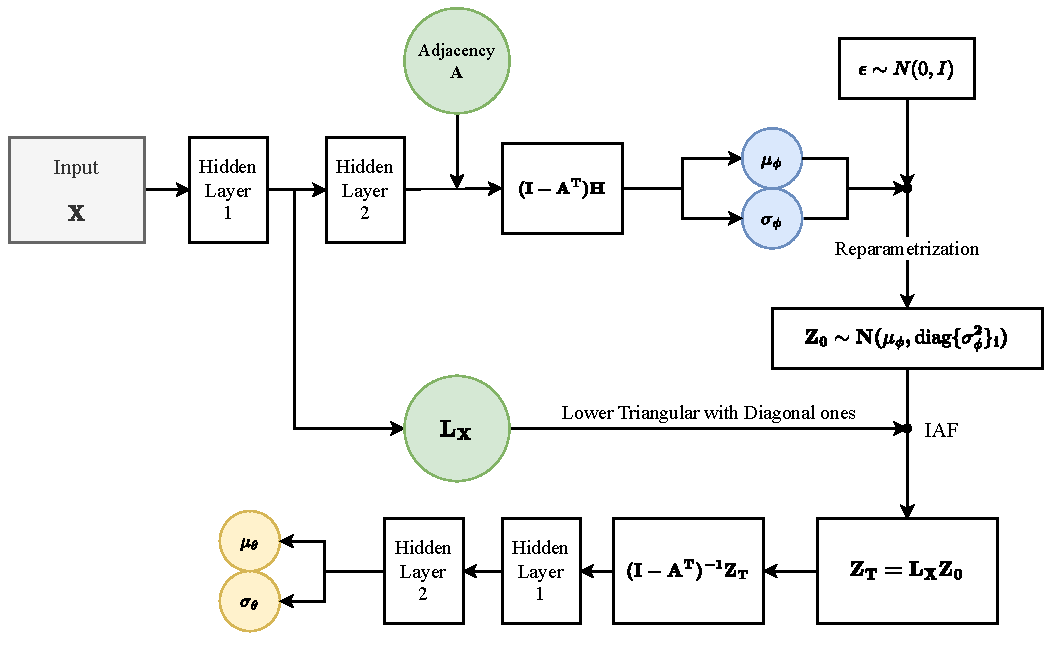
\includegraphics[width=0.9\textwidth]{fig/model.pdf}
    \caption{Architecture of the proposed model.}
    \label{diagram}
\end{figure}

\subsection{Learning}

Our model aims to learn the adjacency matrix of the directed acyclic graph. Instead of regarding the mixed graph as a cyclic graph, we consider them as DAG structure with correlated noise variables. Thus we can use the same optimization procedure as DAG-GNN, which uses the acyclicity constraint as a continuous approximation of the discrete constraint. The optimization procedure is minimizing the following loss function:

\begin{equation}
    \mathcal{L}(A, W, \lambda) =-\mathcal{L}_{\mathrm{ELBO}} + \tau \Vert A \Vert_1 + \lambda h(A) + \frac{c}{2} |h(A)|^2.
\end{equation}

The second term is the L1 regularization term, which encourages sparsity of the adjacency matrix. We found that $\tau=0.1$ works well for a node size of 50. For other node sizes, we use $\tau$ proportional to the inverse of the square of the node size. The third and fourth terms are the augmented Lagrangian terms. We gradually increase the value of $c$ during the training process, as a larger value of $c$ reduces the acyclicity constraint to zero \cite{yu2019daggnn}.


\section{Experiment}

In this section, we conduct experiments on simulated data to evaluate the performance of our proposed method. We compare our method with the DAG-GNN \cite{yu2019daggnn} with random graph datasets. We used a thresholding value of extracting graph as 0.3 which is the same value used at DAG-GNN and NOTEARS.\\ 

\paragraph*{Datasets} Random graph datasets are generated using the following procedure. First, we generate a random directed acyclic graph using the Erdős–Rényi model. In Section 5.1, we consider the case where the noise variables follow not only an independent Gaussian distribution but also independent Laplace and exponential distributions. In Section 5.2, we conduct experiments where the noise variables follows a multivariate Gaussian distribution with a non-diagonal covariance matrix. We randomly select a given proportion of edges and make them bidirectional. Then, we generate a corresponding random covariance matrix and generate multivariate Gaussian data using that covariance matrix. In both sections, we generate 5000 samples for each graph. For the size of the graph, we use 10, 20, 30, and 50 nodes. For the proportion of bidirectional edges, we use 0.1, 0.3, 0.5, and 0.8. \\

\paragraph*{Evaluation} We evaluate the performance of our method using two metrics: Structural Hamming Distance (SHD) and False Discovery Rate (FDR). SHD measures the number of edge additions, deletions, and reversals required to transform the estimated graph into the true graph. FDR represents the ratio of false positives to the total number of predicted edges. These metrics are calculated by comparing the estimated graph with the true graph, considering bidirectional edges. For each combination of the number of nodes and the proportion of bidirectional edges, we generate at least 5 random graphs and calculate the average metrics.

\subsection{Independent Noise Cases}

To compare the performance of our method with DAG-GNN, we conducted experiments on random graphs with independent noise variables. Specifically, we considered cases where the noise variables followed independent Gaussian, Laplace, and exponential distributions. The results of the experiments are shown in Figures \ref*{SHD_FDR_gaussian}, \ref*{SHD_FDR_laplace}, and \ref*{SHD_FDR_exponential}. In the case of Gaussian noise, despite using the original settings of DAG-GNN, the normalizing flow did not show superior performance compared to DAG-GNN. On average, for 10 nodes, our model and DAG-GNN achieved SHD values of 16.5 and 13, respectively. For 20 nodes, the SHD values were 24.7 and 22.1, and for 30 nodes, they were 21.8 and 18.4. However, in the case of non-Gaussian noise, our method consistently outperformed DAG-GNN in terms of both SHD and FDR as the number of nodes increased.

\begin{figure}[H]
    \centering
    \begin{subfigure}{0.3\textwidth}
        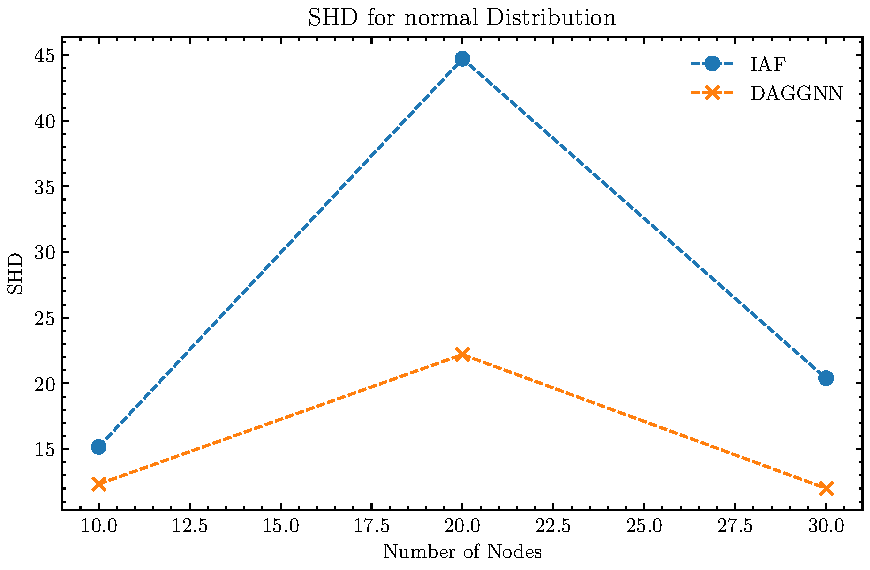
\includegraphics[width=\textwidth]{fig/SHD_independence_normal.pdf}
        \caption{SHD with Gaussian noise}
        \label{SHD_gaussian}
    \end{subfigure}
    \hfill
    \begin{subfigure}{0.3\textwidth}
        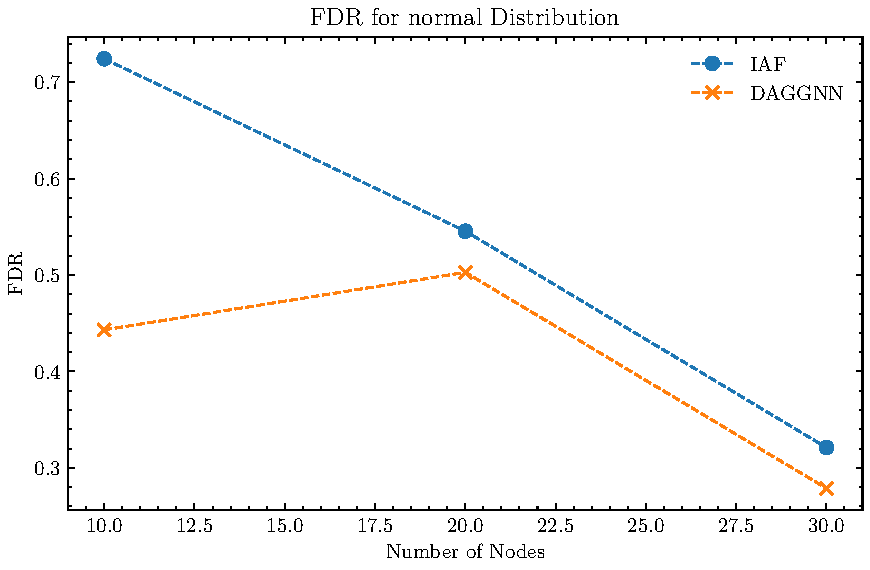
\includegraphics[width=\textwidth]{fig/FDR_independence_normal.pdf}
        \caption{FDR with Gaussian noise}
        \label{FDR_gaussian}
    \end{subfigure}
    \hfill
    \begin{subfigure}{0.3\textwidth}
        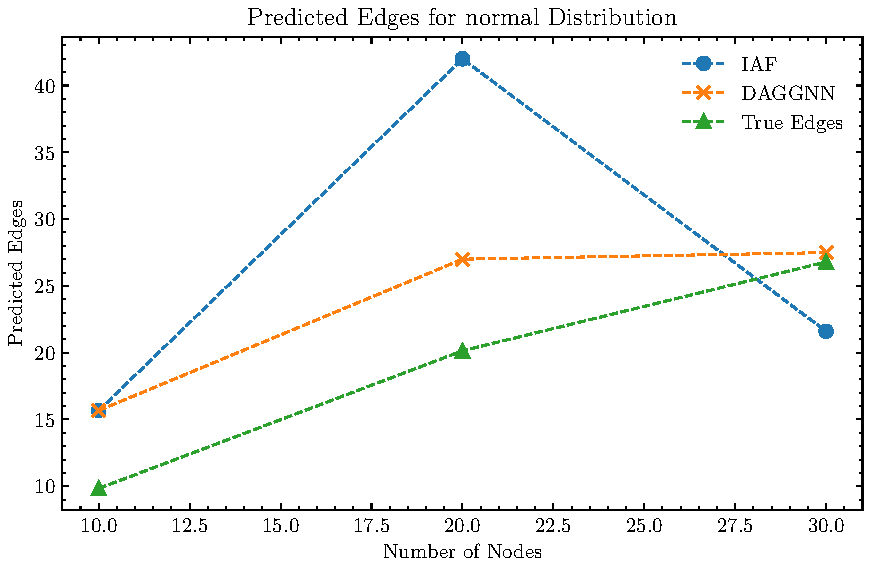
\includegraphics[width=\textwidth]{fig/Predicted Edges_independence_normal.pdf}
        \caption{Number of predicted edges}
        \label{pred_edge_gaussian}
    \end{subfigure}
    \caption{SHD, FDR, and number of predicted edges with independent Gaussian noise}
    \label{SHD_FDR_gaussian}
\end{figure}

In cases where the noise variables follow Laplace or exponential distributions, our method consistently outperformed DAG-GNN in terms of both SHD and FDR. The results of the experiments are shown in Figure \ref*{SHD_FDR_laplace} and \ref*{SHD_FDR_exponential}. As the number of nodes increases, our method consistently demonstrates better performance compared to DAG-GNN in terms of SHD. The FDR values of our method are also lower than those of DAG-GNN, except for the case of 20 with exponential noise.\\

\begin{figure}[H]
    \centering
    \begin{subfigure}{0.45\textwidth}
        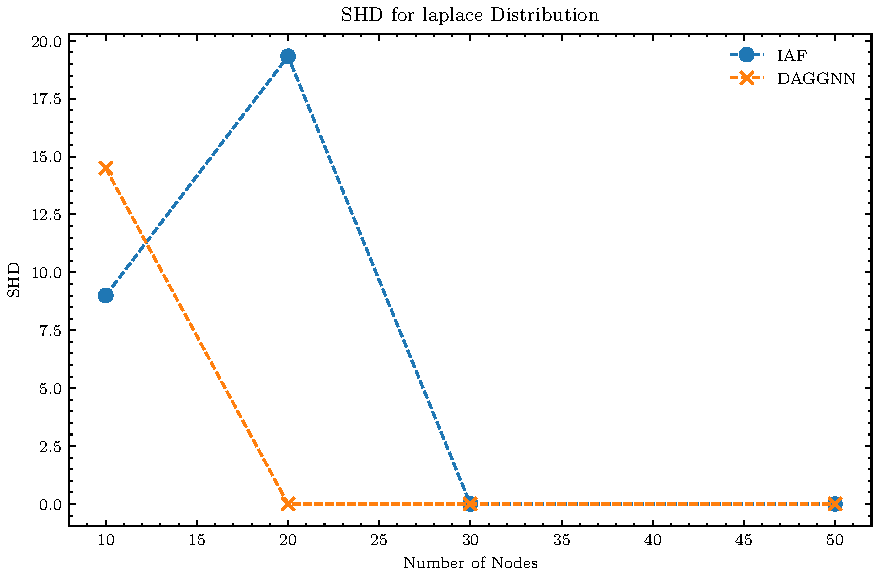
\includegraphics[width=\textwidth]{fig/SHD_independence_laplace.pdf}
        \caption{SHD with Laplace noise}
        \label{SHD_laplace}
    \end{subfigure}
    \hfill
    \begin{subfigure}{0.45\textwidth}
        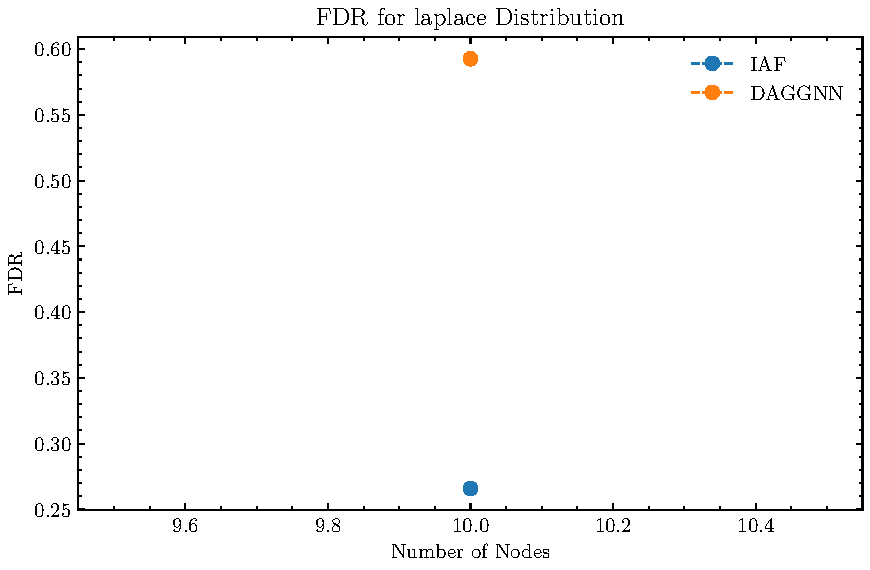
\includegraphics[width=\textwidth]{fig/FDR_independence_laplace.pdf}
        \caption{FDR with Laplace noise}
        \label{FDR_laplace}
    \end{subfigure}
    \caption{SHD and FDR with independent Laplace noise}
    \label{SHD_FDR_laplace}
\end{figure}

\begin{figure}[H]
    \centering
    \begin{subfigure}{0.45\textwidth}
        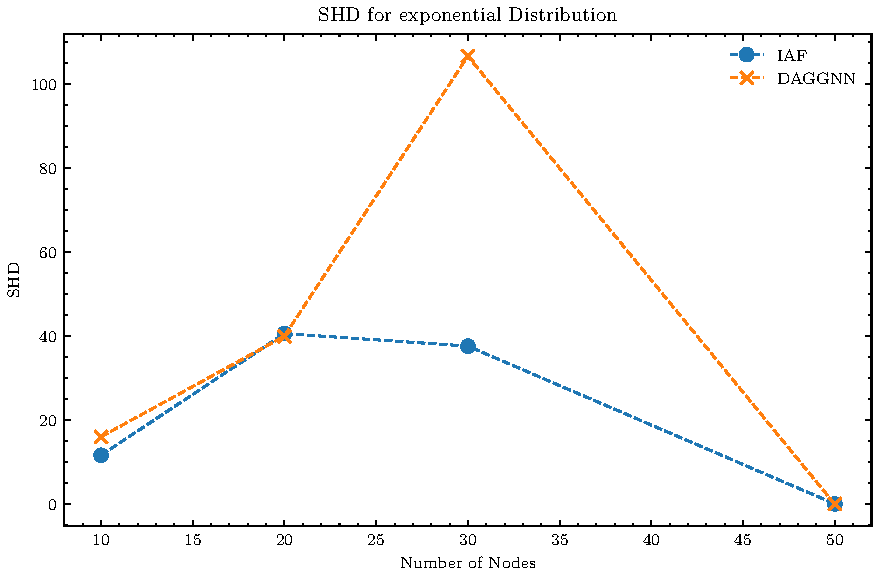
\includegraphics[width=\textwidth]{fig/SHD_independence_exponential.pdf}
        \caption{SHD with exponential noise}
        \label{SHD_exponential}
    \end{subfigure}
    \hfill
    \begin{subfigure}{0.45\textwidth}
        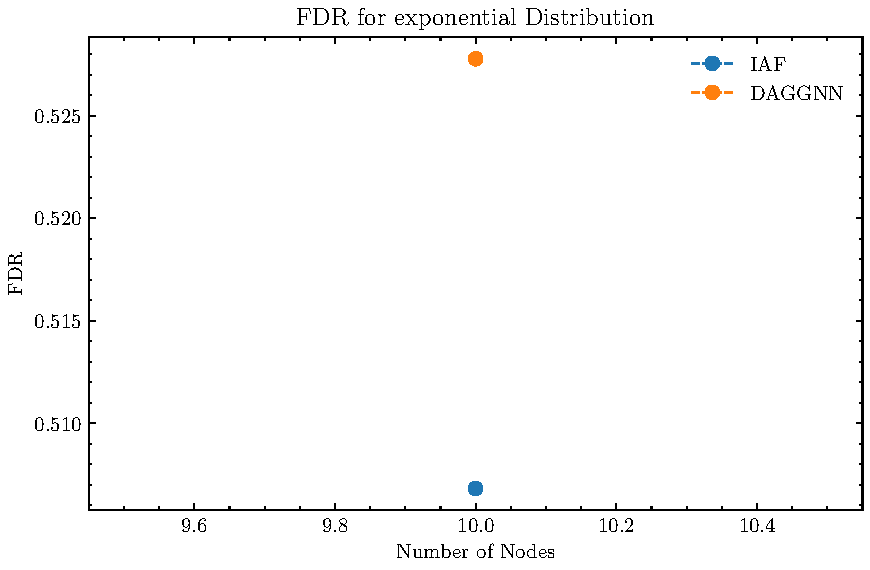
\includegraphics[width=\textwidth]{fig/FDR_independence_exponential.pdf}
        \caption{FDR with exponential noise}
        \label{FDR_exponential}
    \end{subfigure}
    \caption{SHD and FDR with independent exponential noise}
    \label{SHD_FDR_exponential}
\end{figure}

Furthermore, we observed that our method produces a more accurate graph structure than DAG-GNN in cases where the noise variables are independent. As shown in Figure \ref*{pred_edge_laplace_exponential}, the number of predicted edges from both methods is similar when the node size is 10. However, as the node size increases, our method consistently produces a smaller number of predicted edges compared to DAG-GNN. This is in line with our method's superior performance in terms of SHD and FDR. Figure \ref*{example_graphs_indep} presents the estimated graphs produced by each method. The graph estimated by DAG-GNN (third column) contains considerably more edges than the true graph (first column), whereas the graph estimated by our method (second column) has a number of edges much closer to that of the true graph. Therefore, our method not only achieves better performance in terms of accuracy but also provides a more reliable estimation of the true graph structure.\\

\begin{figure}[H]
    \centering
    \begin{subfigure}{0.45\textwidth}
        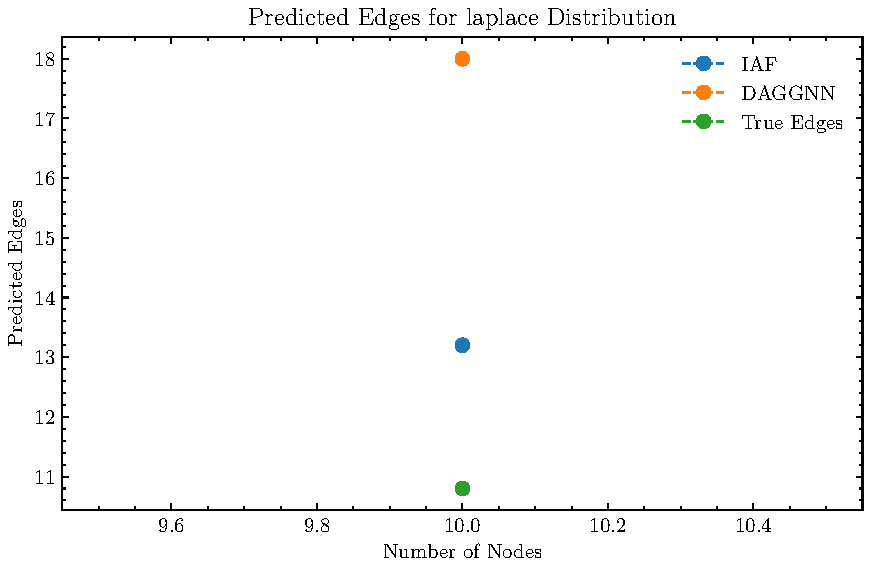
\includegraphics[width=\textwidth]{fig/Predicted Edges_independence_laplace.pdf}
        \caption{Predicted edges with Laplace noise}
        \label{pred_edge_laplace}
    \end{subfigure}
    \hfill
    \begin{subfigure}{0.45\textwidth}
        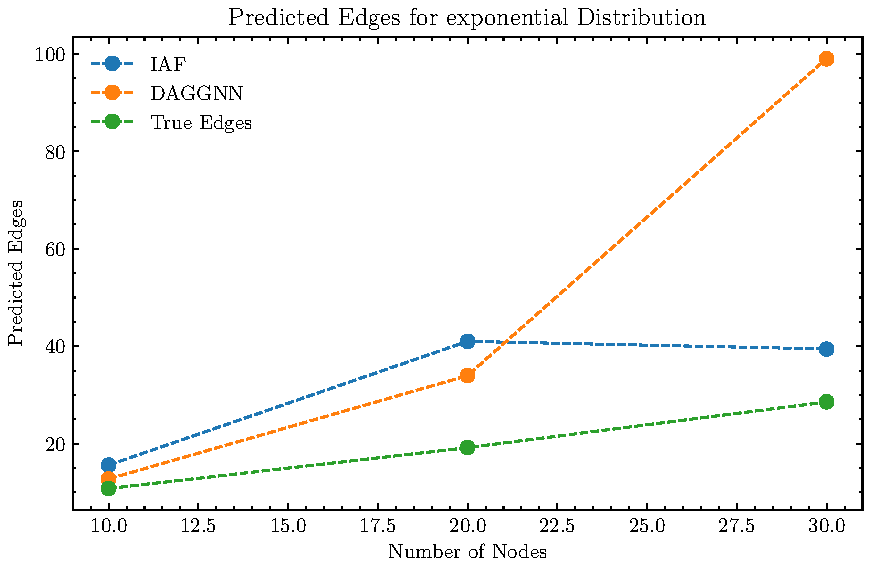
\includegraphics[width=\textwidth]{fig/Predicted Edges_independence_exponential.pdf}
        \caption{Predicted edges with exponential noise}
        \label{pred_edge_exponential}
    \end{subfigure}
    \caption{Number of predicted edges with Laplace and exponential noise}
    \label{pred_edge_laplace_exponential}
\end{figure}

\begin{figure}[H]
    \centering
    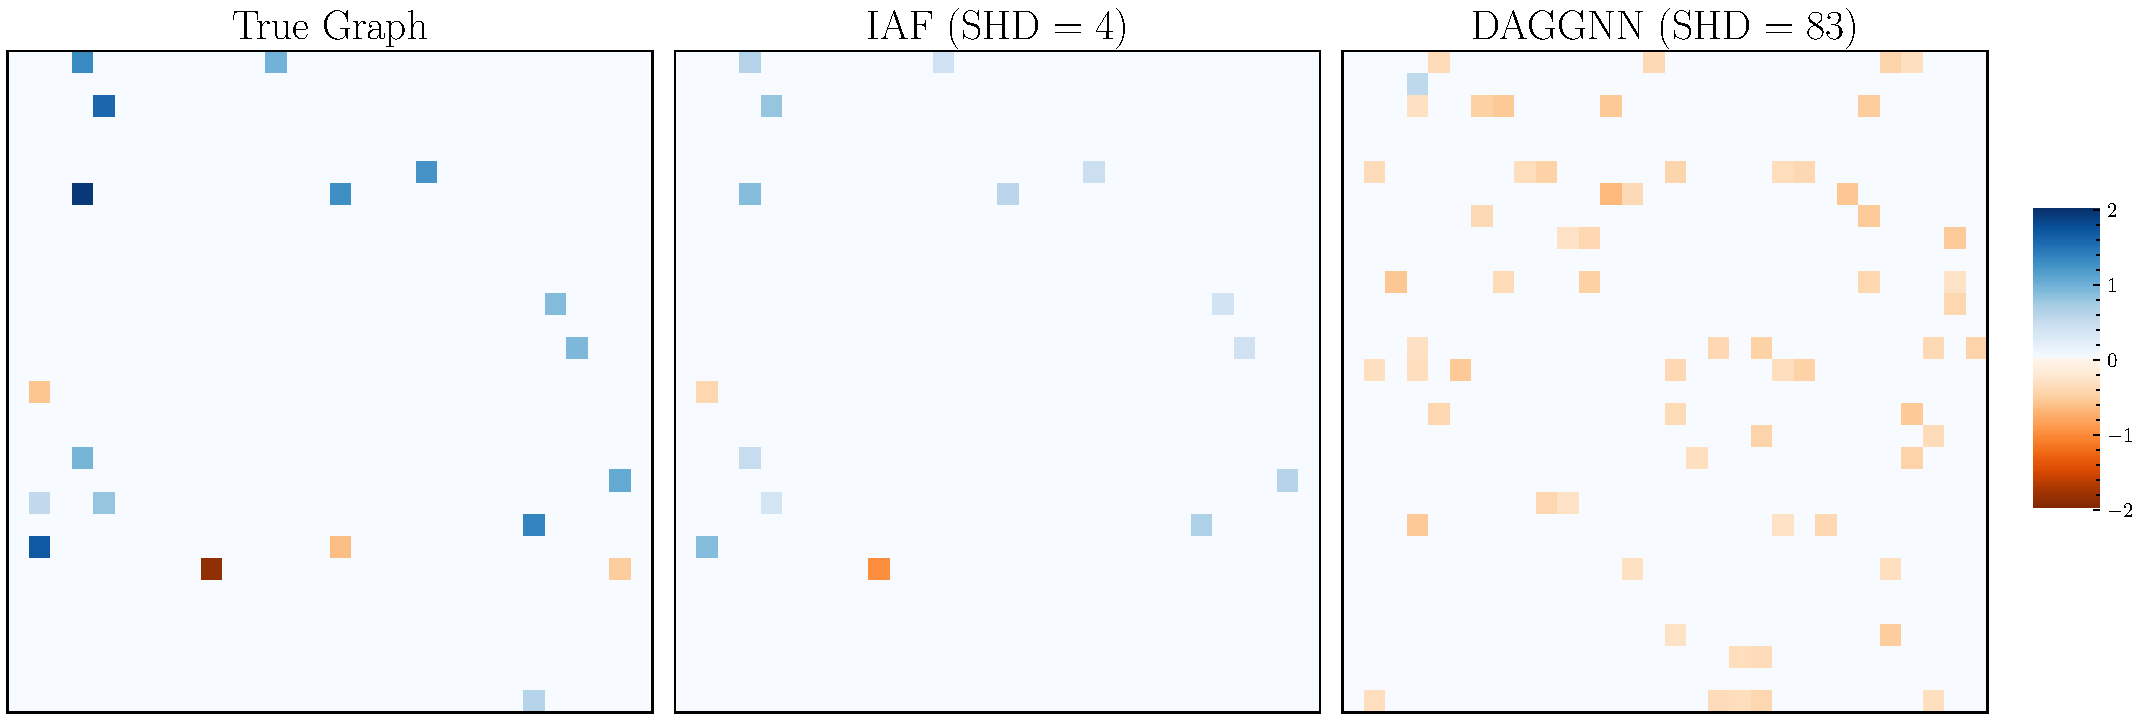
\includegraphics[width=0.8\textwidth]{fig/comparison_indep_30_laplace_seed201.pdf}
    \caption{Example of estimated graphs with node size 30 and exponential noise}
    \label{example_graphs_indep}
\end{figure}

\subsection{Dependent Noise Cases}

To begin with, we set the proportion of bidirectional edges to 0.3 and compared the performance of our method with that of DAG-GNN. The results, as depicted in Figure \ref*{SHD_FDR_prop30}, demonstrate that our method outperforms DAG-GNN in terms of both SHD and FDR. Notably, with a node size of 20, our method exhibited stable training, resulting in a significant difference in SHD and FDR. Figure \ref*{example_graphs} presents the estimated graphs produced by each method. The graph estimated by DAG-GNN (third column) contains considerably more edges than the true graph (first column), whereas the graph estimated by our method (second column) has a number of edges much closer to that of the true graph.\\

\begin{figure}[H]
    \centering
    \begin{subfigure}{0.45\textwidth}
        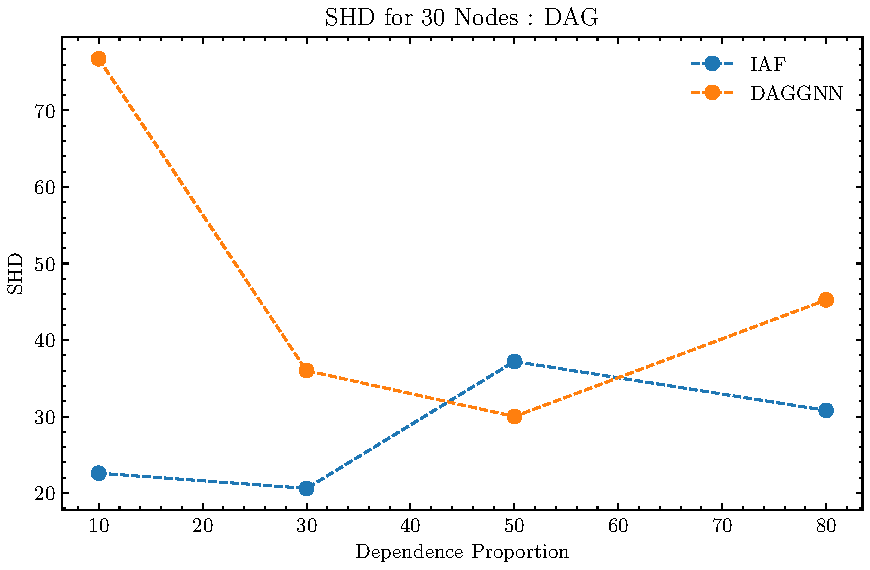
\includegraphics[width=\textwidth]{fig/SHD_dependence_30_DAG_threshold0.3.pdf}
        \caption{SHD with dependence proportion 0.3}
        \label{SHD_prop30}
    \end{subfigure}
    \hfill
    \begin{subfigure}{0.45\textwidth}
        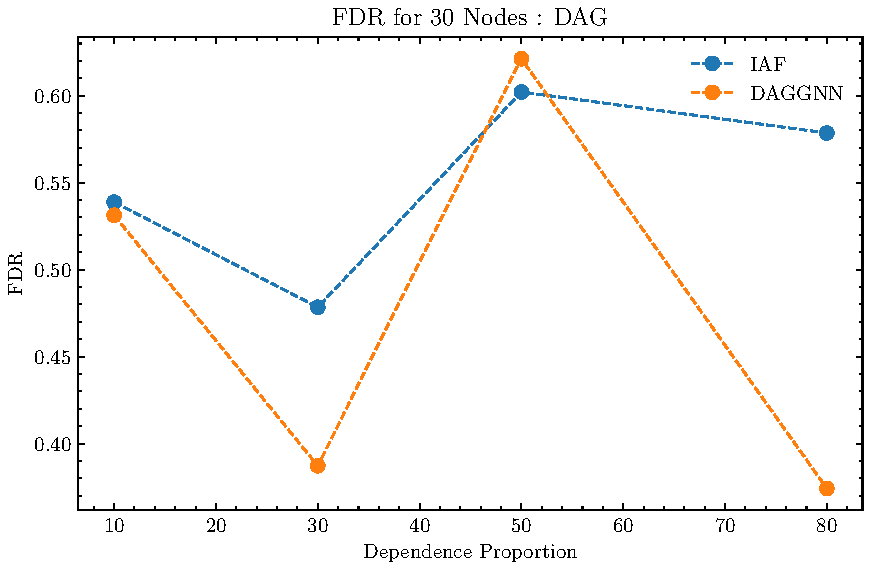
\includegraphics[width=\textwidth]{fig/FDR_dependence_30_DAG_threshold0.3.pdf}
        \caption{FDR with dependence proportion 0.3}
        \label{FDR_prop30}
    \end{subfigure}
    \begin{subfigure}{0.45\textwidth}
        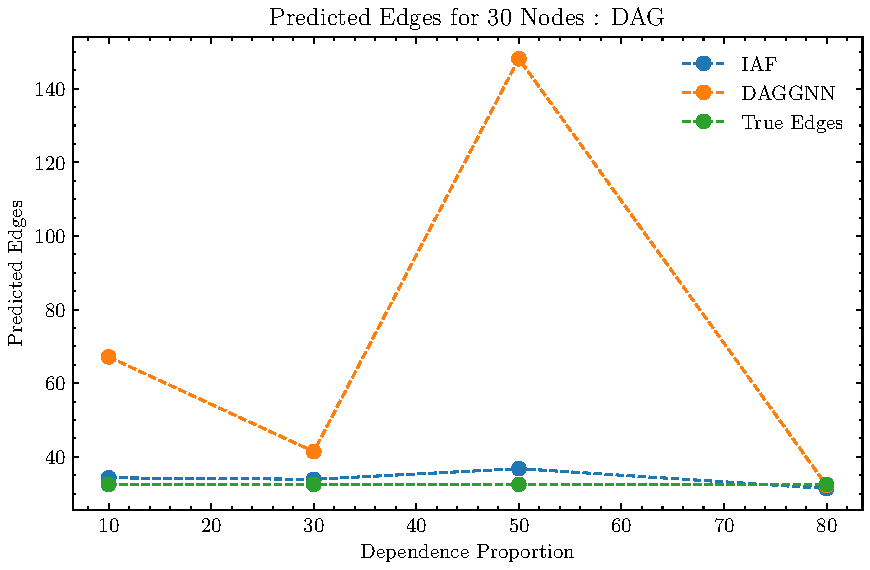
\includegraphics[width=\textwidth]{fig/Predicted Edges_dependence_30_DAG_threshold0.3.pdf}
        \caption{Number of predicted edges}
        \label{pred_edge_prop30}
    \end{subfigure}
    \caption{SHD, FDR, and number of predicted edges with dependence proportion 0.3}
    \label{SHD_FDR_prop30}
\end{figure}

\begin{figure}[H]
    \centering
    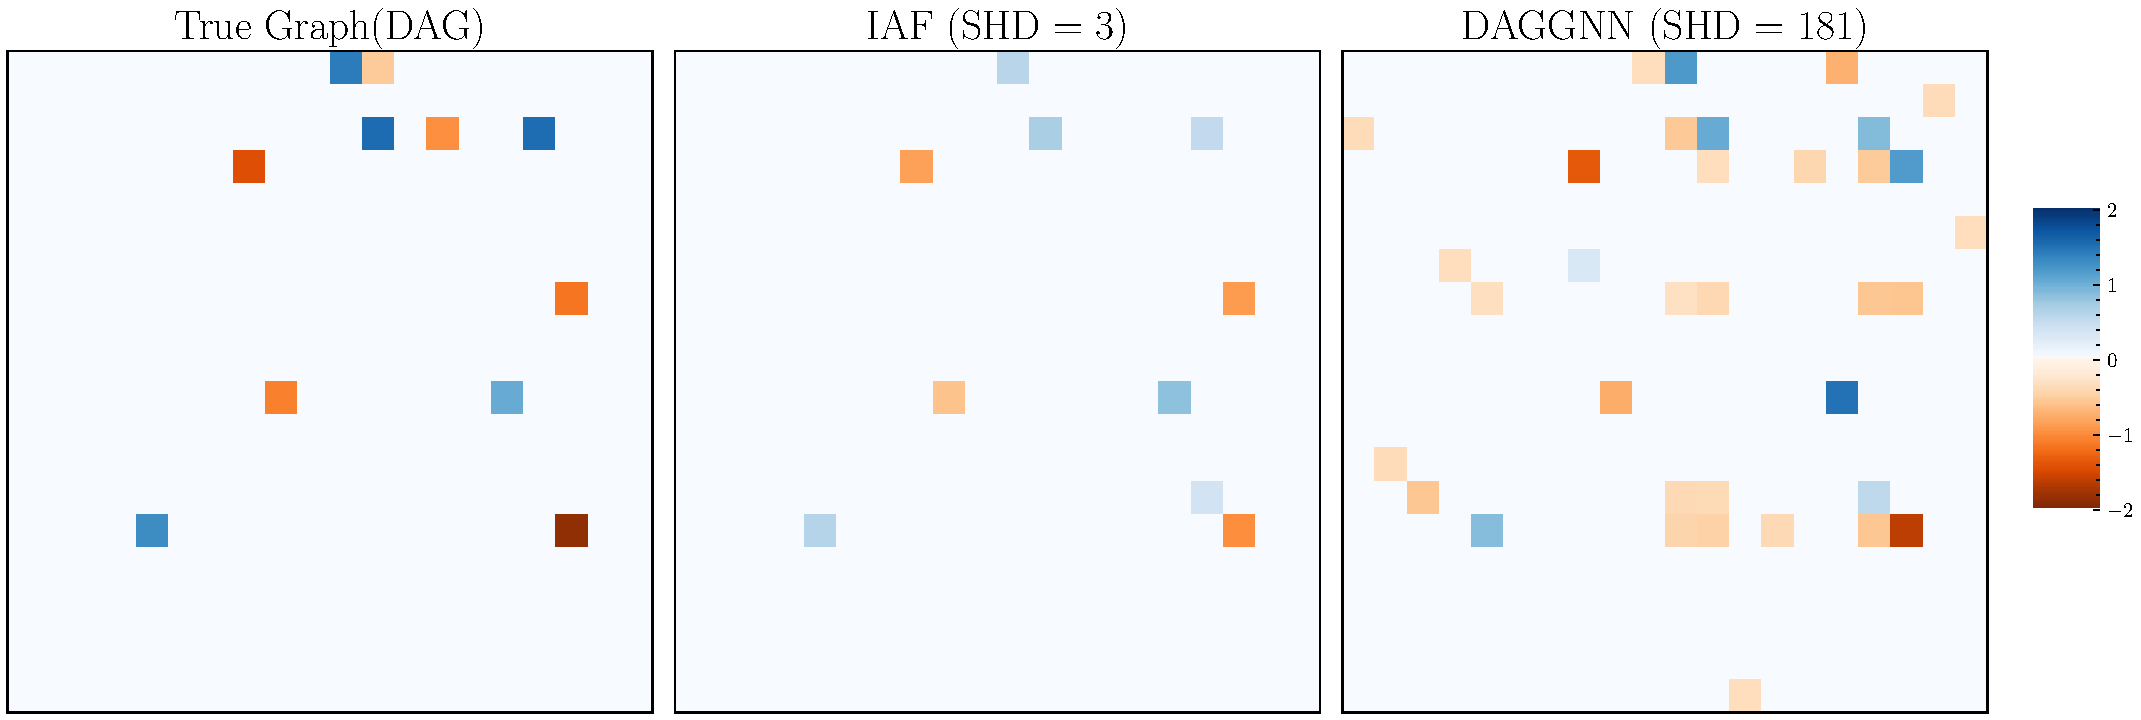
\includegraphics[width=0.8\textwidth]{fig/comparison_dep_20_50_seed31.pdf}
    \caption{Example of estimated graphs with node size 20 and dependence proportion 0.5}
    \label{example_graphs}
\end{figure}

Next, we compare the performance of the two methods, each with varying proportions of bidirectional edges. The results, as illustrated in Figure \ref*{SHD_FDR}, reveal that when the node size is 10, DAG-GNN surpasses our method in terms of SHD. However, when the node size is increased to 20, our method takes the lead, outperforming DAG-GNN in both SHD and FDR metrics.\\

\begin{figure}[p]
    \centering
    \begin{subfigure}{0.45\textwidth}
        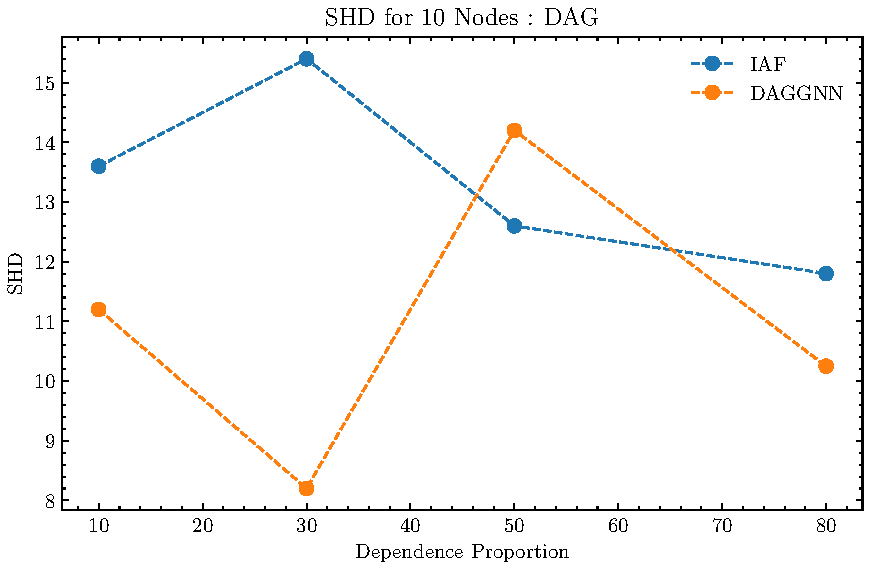
\includegraphics[width=\textwidth]{fig/SHD_dependence_10_DAG_threshold0.3.pdf}
        \caption{SHD with node size 10}
        \label{SHD_node10}
    \end{subfigure}
    \hfill
    \begin{subfigure}{0.45\textwidth}
        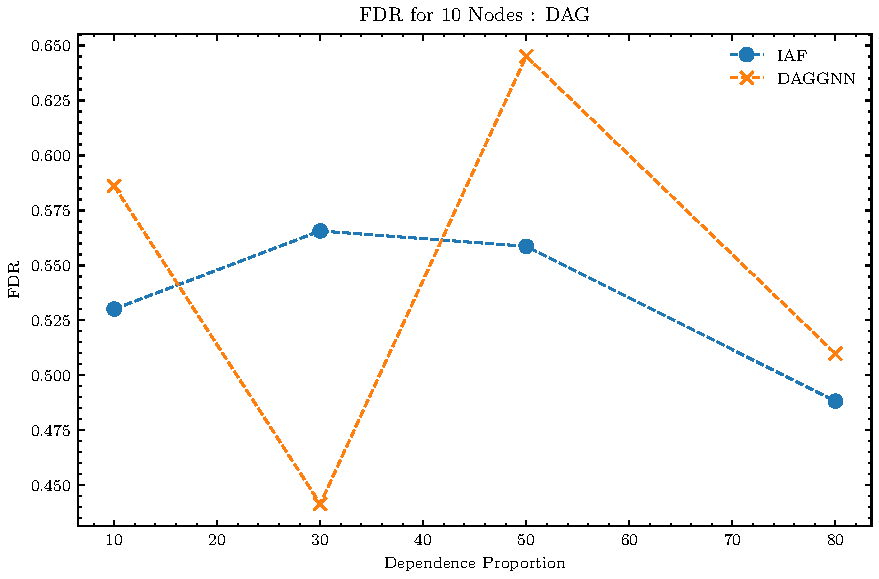
\includegraphics[width=\textwidth]{fig/FDR_dependence_10_DAG_threshold0.3.pdf}
        \caption{FDR with node size 10}
        \label{FDR_node10}
    \end{subfigure}
    \begin{subfigure}{0.45\textwidth}
        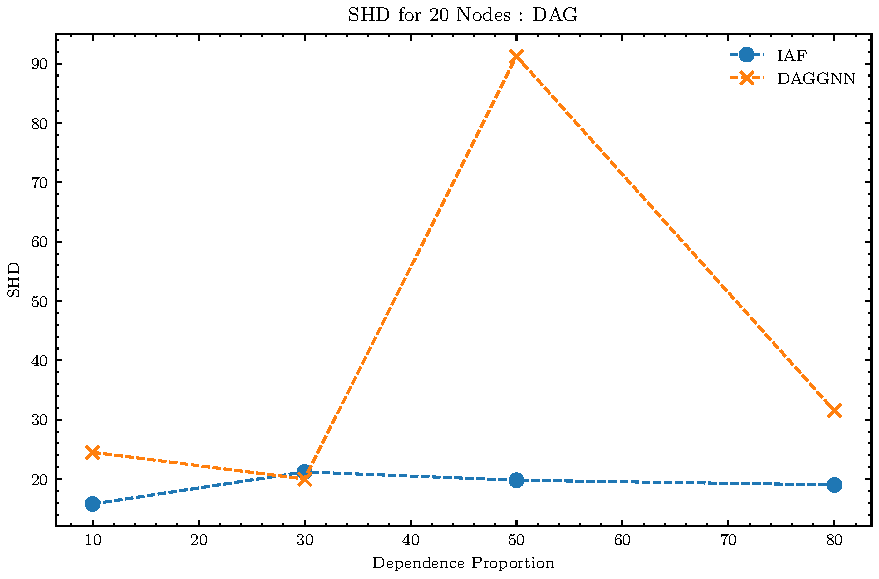
\includegraphics[width=\textwidth]{fig/SHD_dependence_20_DAG_threshold0.3.pdf}
        \caption{SHD with node size 20}
        \label{SHD_node20}
    \end{subfigure}
    \hfill
    \begin{subfigure}{0.45\textwidth}
        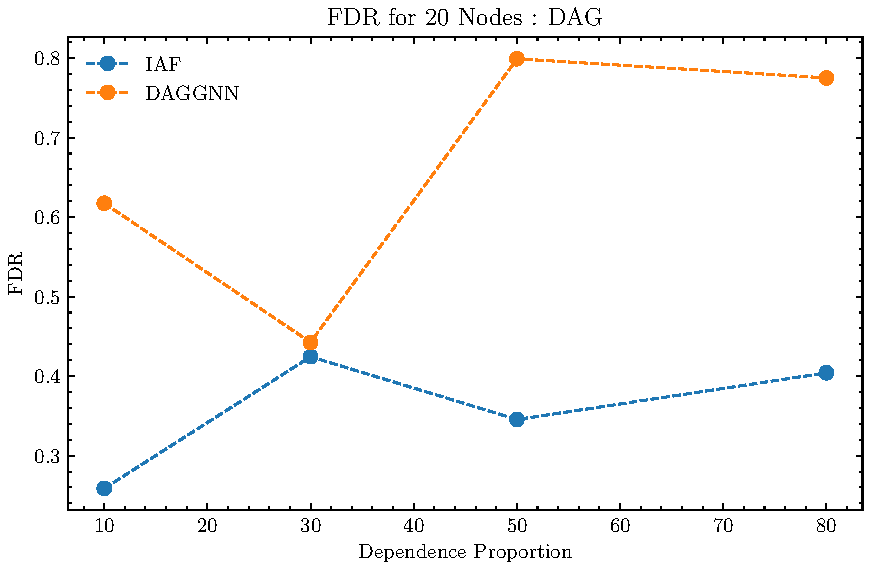
\includegraphics[width=\textwidth]{fig/FDR_dependence_20_DAG_threshold0.3.pdf}
        \caption{FDR with node size 20}
        \label{FDR_node20}
    \end{subfigure}
    \begin{subfigure}{0.45\textwidth}
        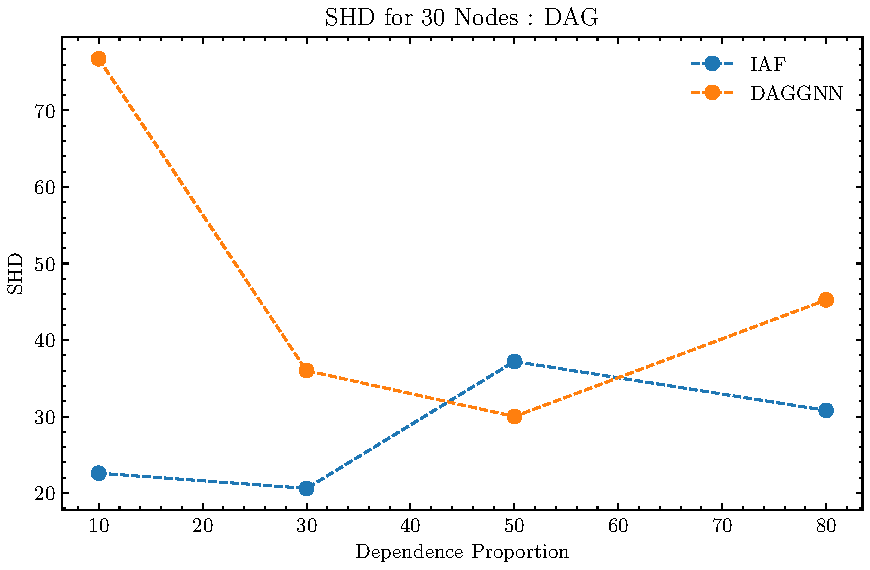
\includegraphics[width=\textwidth]{fig/SHD_dependence_30_DAG_threshold0.3.pdf}
        \caption{SHD with node size 30}
        \label{SHD_node30}
    \end{subfigure}
    \hfill
    \begin{subfigure}{0.45\textwidth}
        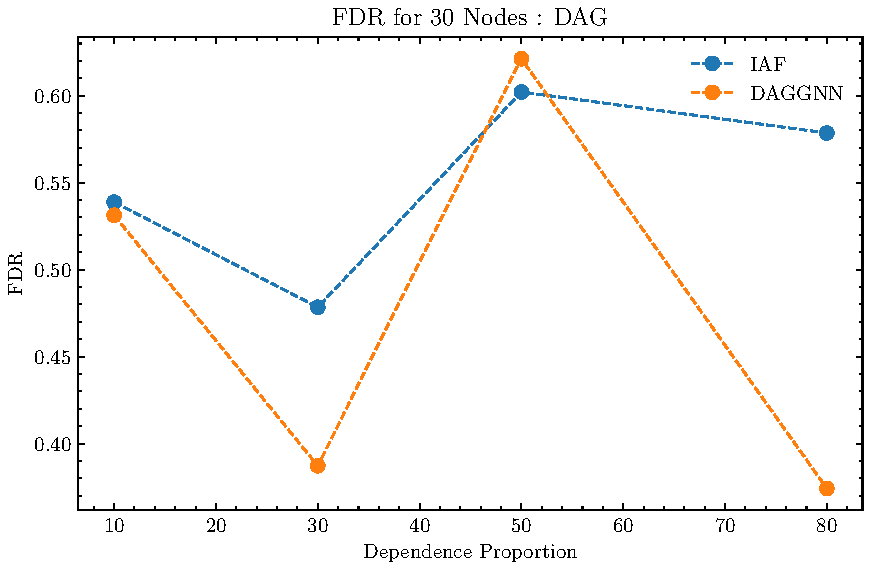
\includegraphics[width=\textwidth]{fig/FDR_dependence_30_DAG_threshold0.3.pdf}
        \caption{FDR with node size 30}
        \label{FDR_node30}
    \end{subfigure}
    \begin{subfigure}{0.45\textwidth}
        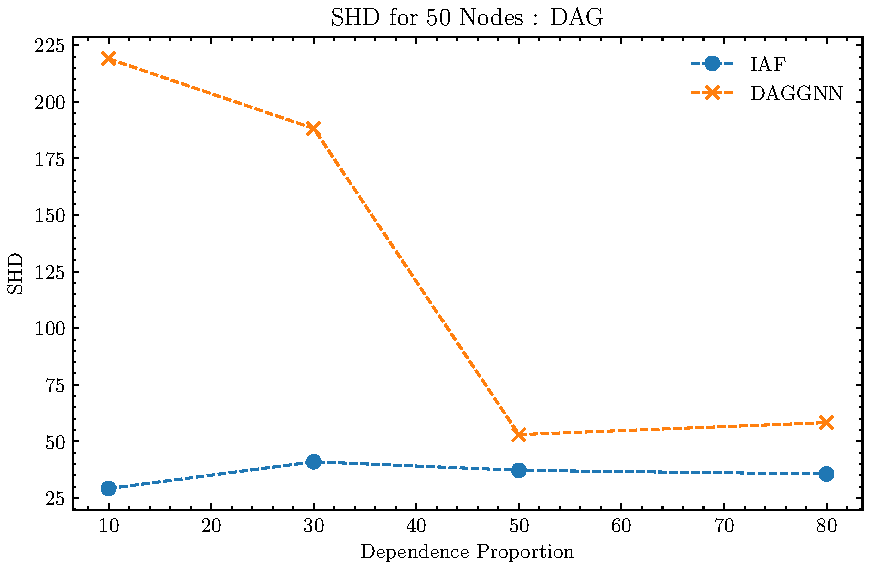
\includegraphics[width=\textwidth]{fig/SHD_dependence_50_DAG_threshold0.3.pdf}
        \caption{SHD with node size 50}
        \label{SHD_node50}
    \end{subfigure}
    \hfill
    \begin{subfigure}{0.45\textwidth}
        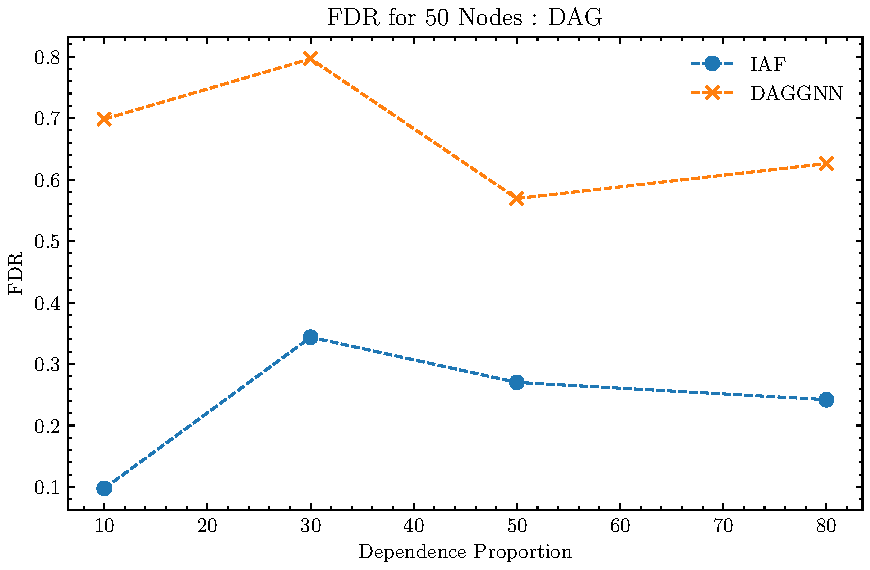
\includegraphics[width=\textwidth]{fig/FDR_dependence_50_DAG_threshold0.3.pdf}
        \caption{FDR with node size 50}
        \label{FDR_node50}
    \end{subfigure}
    \caption{SHD and FDR with dependence proportion 0.1, 0.3, 0.5, and 0.8}
    \label{SHD_FDR}
\end{figure}

In terms of the number of predicted edges, our method consistently produces a number of edges closer to the true number compared to DAG-GNN, especially when the node size is greater than 10. As depicted in Figure \ref*{pred_edge}, the number of predicted edges from both methods are similar when the node size is 10. However, for node sizes 20, 30, and 50, our method consistently produces a number of predicted edges that aligns more closely with the true number of edges compared to DAG-GNN. Considering the better performance of our method in terms of SHD and FDR metrics, we can conclude that our method yields a more accurate graph structure than DAG-GNN.

\begin{figure}
    \centering
    \begin{subfigure}{0.45\textwidth}
        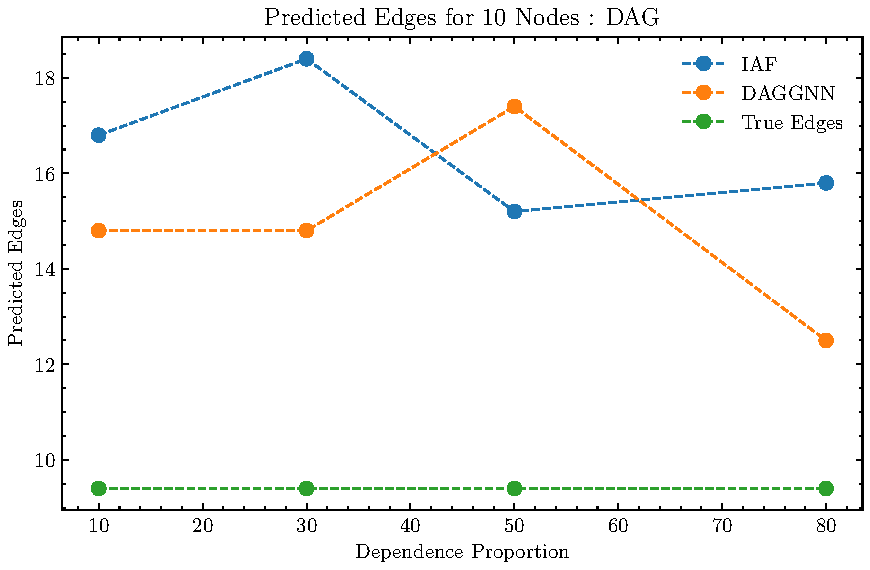
\includegraphics[width=\textwidth]{fig/Predicted Edges_dependence_10_DAG_threshold0.3.pdf}
        \caption{Predicted edges with node size 10}
        \label{pred_edge_node10}
    \end{subfigure}
    \hfill
    \begin{subfigure}{0.45\textwidth}
        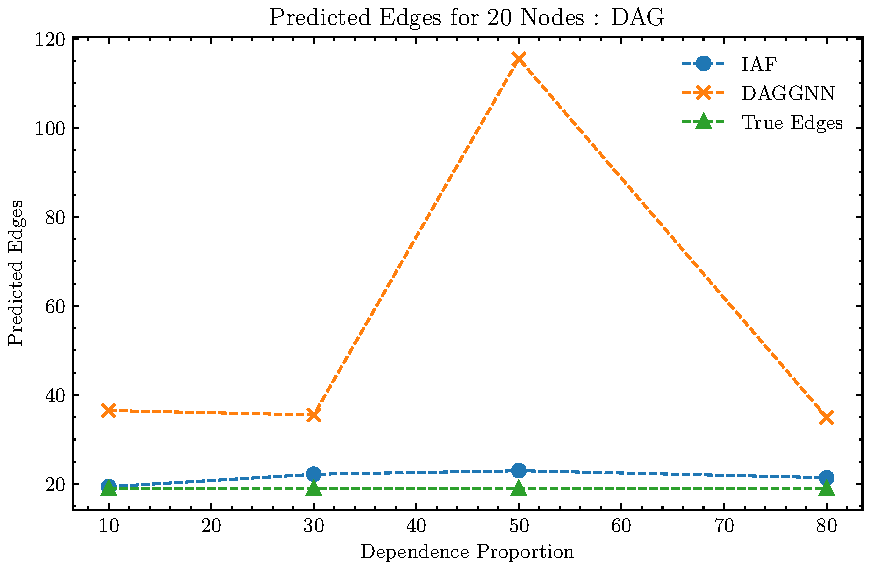
\includegraphics[width=\textwidth]{fig/Predicted Edges_dependence_20_DAG_threshold0.3.pdf}
        \caption{Predicted edges with node size 20}
        \label{pred_edge_node20}
    \end{subfigure}
    \begin{subfigure}{0.45\textwidth}
        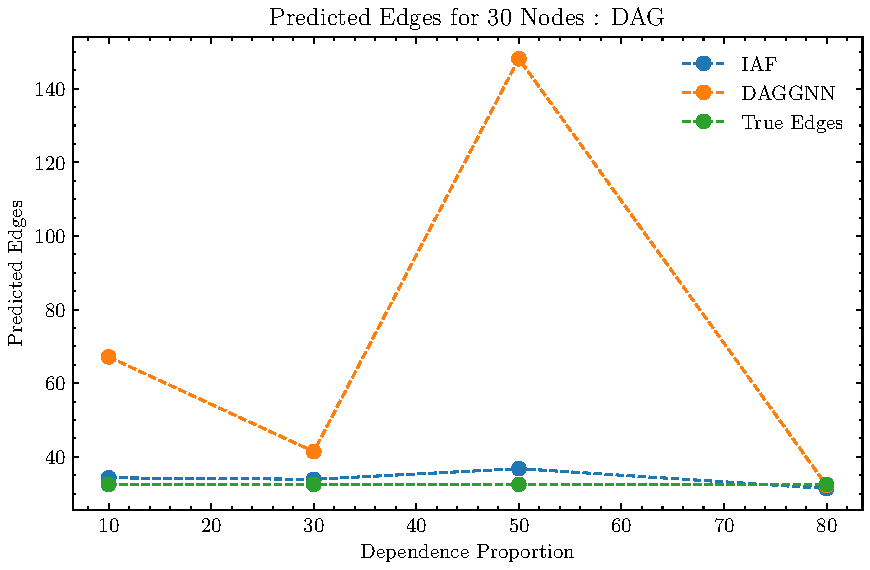
\includegraphics[width=\textwidth]{fig/Predicted Edges_dependence_30_DAG_threshold0.3.pdf}
        \caption{Predicted edges with node size 30}
        \label{pred_edge_node30}
    \end{subfigure}
    \hfill
    \begin{subfigure}{0.45\textwidth}
        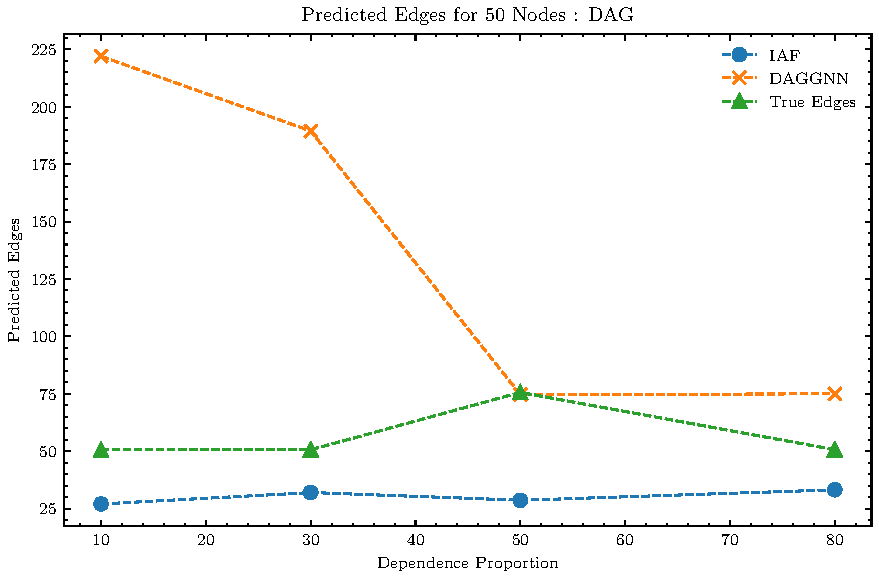
\includegraphics[width=\textwidth]{fig/Predicted Edges_dependence_50_DAG_threshold0.3.pdf}
        \caption{Predicted edges with node size 50}
        \label{pred_edge_node50}
    \end{subfigure}
    \caption{Number of predicted edges with dependence proportion 0.1, 0.3, 0.5, and 0.8}
    \label{pred_edge}
\end{figure}


\section{Conclusion}

In this paper, we proposed a method to learn the structure of a semi-Markovian DAG using a flow-based VAE. We conducted experiments on simulated data and compared the performance of our method with that of DAG-GNN. The results demonstrate that our method outperforms DAG-GNN in terms of both SHD and FDR metrics, especially when the noise variables have dependent structure and when the size of graph is large. In addition, our method produced a number of predicted edges closer to the true number of edges compared to DAG-GNN.\\

However, contrary to our initial expectations, the lower triangular matrix $\mathbf L$ learned in the IAF layer did not capture the covariance matrix of the actual noise variables. This seems to be due to the entanglement problem in the latent space, and resolving this issue remains a future research task. If the full covariance matrix of the noise variables could be found, it could be possible to directly identify bidirectional edges in the graph, enabling more accurate learning of the semi-Markovian graph.

% Biblography
\bibliographystyle{ieeetr}
\bibliography{references}

\end{document}

